\documentclass{article}

\usepackage{pandekten}

\title{Perturbation}
\author{Ch\=an Taku}

\begin{document}

\maketitle

\section{Application in Quantum Mechanics}

This section is from \href{ref/Abbott-Feynman-Diagrams.pdf}{Abbott}.

\begin{proposition}{Feynman Rules for $\phi^3$ Perturbation in Quantum Mechanics}{feynman_rules_for_phi_3_perturbation_in_quantum_mechanics}
    The Feynman rules for
    \[ H_0 = \frac{p^2}{2} + \frac{\omega_0^2 x^2}{2} \]
    with perturbation
    \[ H' = \frac{\lambda x^3}{3!} \]
    is given by the following.
    \begin{itemize}
        \item Propagator:
        \[ 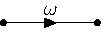
\includegraphics[valign=c]{img/phi3-propagator/phi3-propagator} = \frac{i}{\omega^2 - \omega_0^2 + i\epsilon}. \]
        \item Vertex:
        \[ 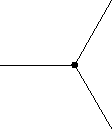
\includegraphics[valign=c]{img/phi3-vertex/phi3-vertex} = -i\lambda. \]
        \item External vertex:
        \[ 
\includegraphics[valign=c]{img/phi3-external/phi3-external} = 1. \]
    \end{itemize}
\end{proposition}

\begin{example}{$\phi^3$ Perturbation in Quantum Mechanics}{phi_3_perturbation_in_quantum_mechanics}
    We evaluate the perturbed expectaion value of $x^2$ using Feynman diagrams by adding up the contributions from diagrams that has two external vertices and no vacuum bubble.
    They are given by
    \begin{align*}
        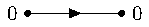
\includegraphics[valign=c]{img/phi3-perturbation/phi3-perturbation.pdf} &= \frac{1}{2\omega_0}; \\
        \frac{1}{2} \times 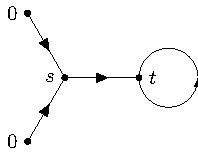
\includegraphics[valign=c]{img/phi3-perturbation/phi3-perturbation2.pdf} &= \frac{1}{2} \frac{\lambda^2}{8\omega_0^6}; \\
        \frac{1}{2} \times 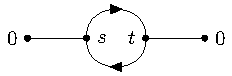
\includegraphics[valign=c]{img/phi3-perturbation/phi3-perturbation3.pdf} &= \frac{1}{2} \frac{\lambda^2}{18\omega_0^6}; \\
        \frac{1}{4} \times 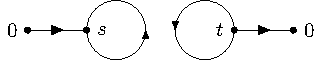
\includegraphics[valign=c]{img/phi3-perturbation/phi3-perturbation4.pdf} &= \frac{1}{4} \frac{\lambda^2}{4\omega_0^6}.
    \end{align*}
    Therefore,
    \[ \bra{\Omega}x^2\ket{\Omega} = \frac{1}{2\omega_0} + \frac{11\lambda^2}{72\omega_0^6}. \]
\end{example}

Note that although the last diagram in the above example is not connected, it contains no vacuum bubble and should therefore be included.
Such graph occurs also in field theory with $\phi^3$ perturbation.
It's contribution to $D(x-y)$ is a constant, i.e. it introduces corrections only to $D(p)$ at $p=0$, and therefore has no physical effect.
\par
Note also that in quantum mechanics, loop diagrams never give divergence results, since
\[ \int \frac{\dd{\omega}}{\omega^2 - \omega_0^2} \]
is free from such problems.
However, such divergence does occur even in $1$-dimensional QFT.

% \bibliographystyle{plain}
% \bibliography{main}

\end{document}
